\documentclass{amsart}

% biber

\usepackage[english]{babel}
\usepackage[utf8]{inputenc}
\usepackage{graphicx}
\usepackage{mathtools}
\usepackage{amsthm}
\usepackage{thmtools,thm-restate}
\usepackage{amsfonts}
\usepackage{hyperref}
\usepackage[backend=biber,url=true,doi=true,eprint=false,style=alphabetic]{biblatex}
\usepackage{enumitem}
\usepackage[justification=centering,singlelinecheck=false]{caption}
\usepackage{indentfirst}
\usepackage{algorithm}
\usepackage{algpseudocode}
\usepackage{listings}
\usepackage[x11names, rgb]{xcolor}
\usepackage{tikz}
\usepackage{hyperref}
\usepackage{subcaption}
\usepackage{booktabs}
\usepackage{linegoal}
\usepackage{csquotes}
\usetikzlibrary{snakes,arrows,shapes}

\addbibresource{references.bib}

\makeatletter
\def\subsection{\@startsection{subsection}{3}%
  \z@{.5\linespacing\@plus.7\linespacing}{.1\linespacing}%
  {\normalfont}}
\makeatother

\makeatletter
\patchcmd{\@setauthors}{\MakeUppercase}{}{}{}
\makeatother

\DeclareMathOperator*{\argmin}{arg\,min}
\DeclareMathOperator*{\argmax}{arg\,max}
\DeclareMathOperator*{\Val}{\text{Val}}
\DeclareMathOperator*{\Ch}{\text{Ch}}
\DeclareMathOperator*{\Pa}{\text{Pa}}
\DeclareMathOperator*{\Sc}{\text{Sc}}
\newcommand{\ov}{\overline}
\newcommand{\region}{\mathcal}

\newcommand\defeq{\mathrel{\overset{\makebox[0pt]{\mbox{\normalfont\tiny\sffamily def}}}{=}}}

\newcommand{\algorithmautorefname}{Algorithm}
\algrenewcommand\algorithmicrequire{\textbf{Input}}
\algrenewcommand\algorithmicensure{\textbf{Output}}
\algrenewcomment[1]{\hspace{0.25cm}\(\triangleright\) #1}
\algnewcommand{\LineComment}[1]{\State\,\(\triangleright\) #1}

\captionsetup[table]{labelsep=space}

\setlistdepth{9}
\newlist{deepitemize}{itemize}{9}
\setlist[deepitemize,1]{label=$\bullet$}
\setlist[deepitemize,2]{label=$\bullet$}
\setlist[deepitemize,3]{label=$\bullet$}
\setlist[deepitemize,4]{label=$\bullet$}
\setlist[deepitemize,5]{label=$\bullet$}
\setlist[deepitemize,6]{label=$\bullet$}
\setlist[deepitemize,7]{label=$\bullet$}
\setlist[deepitemize,8]{label=$\bullet$}
\setlist[deepitemize,9]{label=$\bullet$}

\theoremstyle{plain}

\newcounter{dummy-def}\numberwithin{dummy-def}{section}
\newtheorem{definition}[dummy-def]{Definition}
\newcounter{dummy-thm}\numberwithin{dummy-thm}{section}
\newtheorem{theorem}[dummy-thm]{Theorem}
\newcounter{dummy-prop}\numberwithin{dummy-prop}{section}
\newtheorem{proposition}[dummy-prop]{Proposition}
\newcounter{dummy-corollary}\numberwithin{dummy-corollary}{section}
\newtheorem{corollary}[dummy-corollary]{Corollary}
\newcounter{dummy-lemma}\numberwithin{dummy-lemma}{section}
\newtheorem{lemma}[dummy-lemma]{Lemma}
\newcounter{dummy-ex}\numberwithin{dummy-ex}{section}
\newtheorem{exercise}[dummy-ex]{Exercise}
\newcounter{dummy-eg}\numberwithin{dummy-eg}{section}
\newtheorem{example}[dummy-eg]{Example}

\numberwithin{equation}{section}

\newcommand{\set}[1]{\mathbf{#1}}
\newcommand{\pr}{\mathbb{P}}
\newcommand{\eps}{\varepsilon}
\renewcommand{\implies}{\Rightarrow}

\newcommand{\bigo}{\mathcal{O}}
\newcommand{\verifier}{\mathcal{V}}
\newcommand{\p}{\text{P}}
\newcommand{\np}{\text{NP}}
\newcommand{\conp}{\text{co-NP}}
\newcommand{\true}{\text{true}}
\newcommand{\false}{\text{false}}

\setlength{\parskip}{1em}

\lstset{frameround=fttt,
	numbers=left,
	breaklines=true,
	keywordstyle=\bfseries,
	basicstyle=\ttfamily,
}

\newcommand{\code}[1]{\lstinline[mathescape=true]{#1}}
\newcommand{\mcode}[1]{\lstinline[mathescape]!#1!}
\newcommand{\dset}[1]{\mathcal{#1}}
\newcommand{\ddspn}[2]{\frac{\partial#1}{\partial#2}}
\newcommand{\iddspn}[2]{\partial#1/\partial#2}

\title{%
  \noindent\rule{13cm}{1.0pt}\\
  \vspace{0.2cm}
  A Polynomial-time Reduction of the 3-SAT to the Quadratic Congruence Problem and other Related Problems
  \noindent\rule{13cm}{0.8pt}
}
\xdef\shorttitle{Quadratic congruence polynomial-time reduction}
\author[]{\normalsize Renato Lui Geh\\\small NUSP\@: 8536030\\\\Computational Number Theory
(MAC6927)\\Prof\@. Sinai Robins\\University of São Paulo\\}

\begin{document}

\begin{abstract}
  In this term paper for MAC6927 --- Computational Number Theory, we explore the history behind the
  quadratic congruence problem (QCP) and other related number theoric problems; show a
  polynomial-time reduction from the 3-SAT to the QCP quoting Adleman and Mander's 1978
  theorem~\cite{qcp2}, implying that quadratic congruence is NP-complete; and show some solved and
  unsolved problems in Number Theory that are directly (or indirectly) related to the QCP problem
  and its membership in NP\@.
  \vspace*{-3.5em}
\end{abstract}

\maketitle

\section{History}

German mathematician David Hilbert published~\cite{hilbert} in 1902 a set of 23 unsolved problems
in mathematics he deemed to be most important unanswered mathematical problems of the 20th century.
Since then 9 of them have been solved (at the time the author is writing this line and as far as
the author is aware), 9 are considered partially solved, three of them are unsolved and two of them
are considered too vague. Unsolved problems include the infamous Riemann Hypothesis and an
extension to the Kronecker-Weber Theorem. Amongst solved problems is the 10th Hilbert problem.

\textbf{10th Hilbert Problem:} Given a diophantine equation with any number of unknown quantities
and with rational integral numerical coefficients: \textit{to devise a process according to which
it can be determined by a finite number of operations whether the equation is solvable in rational
integers}.

It was answered in 1970 by Matiyasevich~\cite{diophantine} to be impossible. The question now
becomes, in which cases is there an algorithm for solvability and what is the complexity of such
algorithms? In 1976, Adleman and Manders~\cite{qcp1} partially answered these questions by proving
that, for the quadratic cases, there exists an algorithm and it is NP-complete. In their proof,
they also found that, through a slight modification in the final step of their proof, it was
possible to answer the quadratic congruence problem. A cleaner version of this proof was published
in 1978 by Adleman and Manders~\cite{qcp2}, proof we try to explain in this paper.

In this paper we focus on the second result of Adleman and Mander's 1978 article, but also show the
main result, namely that the set of quadratic diophantine equations with natural numbers solutions
is NP-complete. The proof is done through a polynomial-time reduction from the 3-SAT problem. This
reduction implies that both problems covered in Adleman and Mander's article are in NP-complete.

In 1971, American mathematician Stephen Cook published ``The Complexity of Theorem-proving
Procedures''~\cite{cook}, and in the next year, his fellow countryman Richard Karp published
``Reducibility Among Combinatorial Problems''~\cite{karp}. The two articles introduced the concepts
of P and NP classes, yielding the duo a Turing Award. Interestingly in 1973, on the other side of
the Iron Curtain, Ukrainian Leonard Levin published~\cite{levin} in the USSR equivalent results to
Cook's and Karp's, but considering search problems instead of decision problems (an interesting
remark is that Levin did not receive a Turing Award for his work, despite having achieved
equivalent results). Both works resulted in the following statement: that any problem in NP can be
reduced in polynomial time by a deterministic Turing machine to the problem of satisfiability of a
Boolean formula, i.e.\ the SAT problem.  Additionally, if there exists a deterministic polynomial
time algorithm for solving SAT, then every NP problem can be solved by a deterministic polynomial
time algorithm.

This independent, parallel work from opposite parts of the world, ideologically and geographically,
gave rise to what is considered one of the most important open questions in theoretical computer
science, the P vs NP problem.

\begin{deepitemize}
  \item Satisfiability (SAT)
    \begin{deepitemize}
      \item 0--1 integer programming
      \item Clique
        \begin{deepitemize}
          \item Set packing
          \item Vertex cover
            \begin{deepitemize}
              \item Set covering
              \item Feedback node set
              \item Feedback arc set
              \item Directed Hamiltonian cycle
                \begin{deepitemize}
                  \item Undirected Hamiltonian cycle
                \end{deepitemize}
            \end{deepitemize}
        \end{deepitemize}
      \item Satisfiability with at most 3 literals per clause (3-SAT)
        \begin{deepitemize}
          \item Chromatic number
            \begin{deepitemize}
              \item Clique cover
              \item Exact cover
                \begin{deepitemize}
                  \item Hitting set
                  \item Steiner set
                  \item 3-dimensional matching
                  \item Knapsack
                    \begin{deepitemize}
                      \item Job sequencing
                      \item Partition
                        \begin{deepitemize}
                          \item Max cut
                        \end{deepitemize}
                    \end{deepitemize}
                \end{deepitemize}
            \end{deepitemize}
        \end{deepitemize}
    \end{deepitemize}
\end{deepitemize}

In his 1972 paper, Karp also published a list of 21 NP-complete problems in which he showed
reductions implying its membership in the NP-complete class. The list above is Karp's 21
NP-complete problems, where the nesting indicates the direction of the reduction. For instance, the
exact cover problem was reduced to the knapsack problem, chromatic number was reduced to exact
cover, 3-SAT was reduced to exact cover, and the SAT was reduced to the 3-SAT problem.

From this we know that the 3-SAT is NP-complete. Not only that, any problem that is reduces
3-SAT is also in NP\@. In the next sections we will provide a brief review on polynomial-time
reductions, present proper definitions on the QCP and 3-SAT, and prove the reduction. This section
provided a brief historical overview, but we do not restrict historical remarks to only this
section. When relevant, we provide short historical anecdotes on the subject.

\section{Brief Review on Complexity Theory}

In this section we define decision problems, the P and NP complexity classes and all the tools we
need to prove a polynomial-time reduction. We give a shallow definition of the 3-SAT problem and
give other examples of NP-complete problems.

Before we prove reductions, we first need to properly define the concepts we are going to use. We
shall define a Problem as a question that takes a set of objects as input and returns another set
of objects as output. There are many types of problems: decision problems, where the output is
restricted to yes or no (or true or false) answers; optimization problems, where the answer is
given by a particular element of a set such that such an object optimizes certain criteria; and
search problems, which is when the answer is an element of the set of output answers.

We can give a format for problems:

\begin{algorithm}[h]
  \caption*{\textbf{Problem:} vector sorting}
  \begin{algorithmic}[1]
    \Require\, $n\in\mathbb{N}$ and a vector $A[1..n]$ with $n$ integers
    \Ensure\, An ordered vector
    \Statex\, Sorting the vector $A$ in increasing order.
  \end{algorithmic}
\end{algorithm}

It is natural to conclude that problems have a certain complexity attached to them. Furthermore, we
can provide several algorithms that take the same input and yield the same output. In this case in
particular we know that sorting a vector is $\bigo(n\ln n)$ at best. Examples of algorithms for the
above problem are InsertSort, MergeSort and BubbleSort, with each one having different worst case
complexities. We next show a few examples of different types of problems:

\begin{algorithm}[h]
  \caption*{\textbf{Search problem:} greatest common divisor}
  \begin{algorithmic}[1]
    \Require\,$a, b\neq 0\in\mathbb{N}$
    \Ensure\, $d|a$, $d|b$, and for all $d'|a$, $d'|b$ we have $d'\leq d$
    \Statex\, Finding the $\gcd(a, b)$
  \end{algorithmic}
\end{algorithm}

The Euclidean algorithm is an example of an algorithm that solves the gcd problem, with
$\bigo(\ln(\max\{a,b\}))$.

\begin{algorithm}[h]
  \caption*{\textbf{Optimization problem:} longest common subsequence}
  \begin{algorithmic}[1]
    \Require\, Two strings $X[1..m]$ and $Y[1..n]$
    \Ensure\, A string
    \Statex\, Finding the longest common subsequence in $X$ and $Y$.
  \end{algorithmic}
\end{algorithm}

This classic computer science problem turns out to be $\Theta(m\cdot n)$. Following Cook and
Karp's, we treat only the case for decision problems. One might think this severly restricts the
generality of complexity classes, but it is easy to see that one can treat optimization and search
problems as special cases of decision problems. We do this by restricting these problems into their
decision problem subsets:

\begin{algorithm}[h]
  \caption*{\textbf{Decision problem:} greatest common divisor}
  \begin{algorithmic}[1]
    \Require\,$a, b\neq 0\in\mathbb{N}$ and $k\in\mathbb{N}$
    \Ensure\, Boolean value
    \Statex\, Is $\gcd(a, b)=k$ true?
  \end{algorithmic}
\end{algorithm}

\begin{algorithm}[h]
  \caption*{\textbf{Decision problem:} longest common subsequence}
  \begin{algorithmic}[1]
    \Require\, Two strings $X[1..m]$ and $Y[1..n]$
    \Ensure\, Boolean value
    \Statex\, Is there an LCS of X and Y such that its length $\geq k$?
  \end{algorithmic}
\end{algorithm}

We simply added a $k$ restriction on the input and modified the question so that the answer is a
yes or no question.

For the next part we assume Turing machines to be already defined, as we wish to keep this section
brief, as the title says. We consider an algorithm a series of steps that can be performed by a
Turing machine. A problem is solvable in polynomial time if there exists an algorithm that takes a
polynomial number of steps on the size of the instance. We define an instance as a particular input
of a problem. In the $\gcd$ decision problem, we could take the tuple $(253, 37, 1)$ as an instance
of the input. Both the Euclidean algorithm and the optimal 2-dimension LCS algorithm run in
polynomial time on the size of the instance. However, the general case of the LCS algorithm is
$\bigo(2^{n_1})$, where $n_i$ is the length of the $i$-th string, and thus is not polynomial.

\begin{definition} The P class is the set of all decision problems that can be solved by polynomial
  (on the size of the instance) time algorithms.
\end{definition}

Let $\Pi$ be a Problem. We say that $\Pi$ admits a polynomial verifier $\verifier$ for a YES answer
if there exists a polynomial algorithm that takes an instance $I$ of $\Pi$ and an object
$\mathcal{C}$ such that the size of $\mathcal{C}$ is polynomial and returns YES for some
$\mathcal{C}$ if the answer $\Pi(I)$ is YES and NO for all $\mathcal{C}$ if $\Pi(I)$ is NO\@.

In other words, $\verifier$ takes an instance $I$ and checks whether such an instance is a true
answer to the problem. We call the object $\mathcal{C}$ a polynomial certificate of problem $\Pi$.

Analogally, a polynomial verifier for a NO answer takes a polynomial certificate $\mathcal{C}$ and
returns NO if the answer $\Pi(I)$ is NO and YES for all $\mathcal{C}$ if $\Pi(I)$ is YES\@.

\begin{algorithm}[h]
  \caption*{\textbf{Problem:} Hamiltonian cycle}
  \begin{algorithmic}[1]
    \Require\, A graph $G=(V, E)$
    \Ensure\, Boolean value
    \Statex\, Is there a Hamiltonian cycle, i.e.\ a path $p=(e_1,e_2,\ldots,e_k)$ s.t. $\forall v
    \in V$, $v$ is visited by $p$ exactly once, and $p$ is a cycle?
  \end{algorithmic}
\end{algorithm}

Consider the Hamiltonian cycle problem above. In the image below, the polynomial certificate is the
red path, and the polynomial verifier is an algorithm that checks whether the instance given is an
actual solution to the problem. It is easy to see that a polynomial verifier for the Hamiltonian
cycle is an algorithm that checks whether the set of edges in $\mathcal{C}$ traverse all the
vertices and that the edges form a cycle.

\begin{figure}[h]
  \centering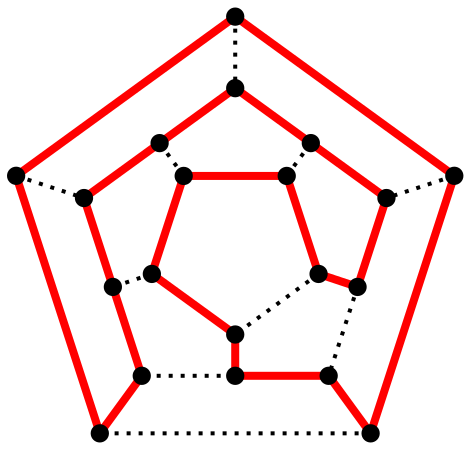
\includegraphics[scale=0.3]{graphs/hamiltonian.png}
  \caption{The red path is a polynomial certificate for the Hamiltonian cycle problem. Source:
  Wikipedia.}
\end{figure}

\begin{definition} The NP class is the set of all decision problems that admit a polynomial
  verifier for the YES answer.
\end{definition}

\begin{definition} The co-NP class is the set of all decision problems that admit a
  polynomial verifier for the NO answer.
\end{definition}

Note how every problem in P is already in NP and co-NP, since the algorithm that solves the problem
could be used as a verifier for both the YES and NO answer.

Let $\Pi$ and $\Pi'$ be problems. A polynomial-time reduction from $\Pi$ to $\Pi'$ is an algorithm
that solves $\Pi$ using an algorithm that solves $\Pi'$ as a subroutine, and that, excluding its
subroutine, is polynomial on the size of its instance. We denote such a reduction by
$\Pi\leq_p\Pi'$ if there exists a polynomial reduction, from $\Pi$ to $\Pi'$.

\begin{algorithm}[h]
  \caption*{\textbf{Problem:} SAT}
  \begin{algorithmic}[1]
    \Require\, A Boolean formula with $n$ variables written in CNF, e.g.\ $(x_1\vee x_2\vee x_2\vee
    x_3)\wedge (\ov{x}_2\vee x_5)\wedge\cdots$
    \Ensure\, Boolean value
    \Statex\, Is there a valuation $\nu :\{x_1,x_2,\ldots,x_n\}\to\{\false, \true\}$ such that the
    input formula evaluates to true?
  \end{algorithmic}
\end{algorithm}

\begin{algorithm}[h]
  \caption*{\textbf{Problem:} 3-SAT}
  \begin{algorithmic}[1]
    \Require\, A Boolean formula with $n$ variables written in CNF with at most 3 literals in each
    clause, e.g.\ $(x_1\vee x_2\vee x_3)\wedge(\ov{x}_2\vee\ov{x}_1\vee x_5) \wedge\cdots$
    \Ensure\, Boolean value
    \Statex\, Is there a valuation $\nu :\{x_1,x_2,\ldots,x_n\}\to\{\false, \true\}$ such that the
    input formula evaluates to true?
  \end{algorithmic}
\end{algorithm}

We can prove that SAT $\leq_p$ 3-SAT by turning the clauses in the SAT problem into 3-SAT
clauses~\cite{karp}. Recall Karp's 23 NP-complete list of problems. Each nesting means that the
nested item $\Pi'$ and its parent item $\Pi$ obey $\Pi\leq_p\Pi'$. The SAT problem, can also be
reduced to the Hamiltonian cycle problem by turning edges and vertices into SAT clauses. The vertex
cover problem can also be reduced to the Hamiltonian cycle problem~\cite{karp}.

\begin{definition} A problem $\Pi$ in NP is NP-complete if $\forall$ $\Pi' \in \np$,
  $\Pi'\leq_p\Pi$.
\end{definition}

From the Cook-Levin Theorem~\cite{cook,levin}, we know that the SAT problem is NP-complete. So if
$\Pi\leq_p\Pi'$, and $\Pi$ is NP-complete, then $\Pi'$ is also NP-complete. So showing that a
problem $\Pi'$ is NP-complete consists of the following steps:

\begin{enumerate}
  \item Take $\Pi'\in \np$,
  \item Take $\Pi$ NP-complete,
  \item Show that $\Pi\leq_p\Pi'$.
\end{enumerate}

\begin{definition} A problem $\Pi$ is NP-hard if the existence of a polynomial algorithm for $\Pi$
  implies on $\p=\np$.
\end{definition}

So every NP-complete problem is NP-hard, but an NP-hard problem is not necessarily in NP\@.

We wish to show that the 3-SAT problem can be reduced to the quadratic congruence problem, proving
that QCP is NP-complete.

\section{The Reduction}



%--------------------------------------------------------------------------------------------------

\printbibliography[]

\end{document}
